\documentclass[11pt,letterpaper]{article}
\usepackage{../assets/scientific_report}
\usepackage{float}
\usepackage{listings}
\usepackage{xcolor}
\usepackage{graphicx}
\usepackage{geometry}
\geometry{headheight=23pt, top=2cm, bottom=2cm, left=2.5cm, right=2.5cm}
\setlength{\parskip}{0.5em}
\setlength{\parindent}{0pt}

\lstset{
    language=C,
    basicstyle=\ttfamily\small,
    keywordstyle=\color{blue}\bfseries,
    commentstyle=\color{green!60!black}\itshape,
    stringstyle=\color{red!80!black},
    numbers=left,
    numberstyle=\tiny\color{gray},
    numbersep=8pt,
    frame=single,
    breaklines=true,
    captionpos=b,
    tabsize=4,
    showstringspaces=false
}

\begin{document}
\pagestyle{plain}

\begin{center}
    {\LARGE\bfseries Estimativa estocástica de $\pi$ com OpenMP}\\[0.4em]
    {\normalsize Eugênio Vitor Lopes dos Santos}\\[0.3em]
    {\small DCA3703 -- Programação Paralela, Universidade Federal do Rio Grande do Norte}\\[0.3em]
\end{center}

\section{Enunciado}
Implementar em C uma estimativa de $\pi$ pelo método de Monte Carlo. O programa deve sortear pontos em um quadrado de lado 2 e contar os que pertencem ao círculo unitário. A atividade pede a paralelização do laço principal com OpenMP, a identificação de uma condição de corrida no contador e duas formas de correção: uma seção \texttt{critical} a cada incremento e um acumulador local por thread. Também são exploradas as cláusulas \texttt{shared}, \texttt{private}, \texttt{firstprivate}, \texttt{lastprivate} e \texttt{default(none)}.

\section{Fundamentação teórica}

\subsection{Método de Monte Carlo}
O quadrado tem área 4 e o círculo unitário tem área $\pi$. Se os pontos forem uniformes no quadrado, a fração de pontos dentro do círculo se aproxima da razão entre as áreas:
\[
\frac{n_{\text{dentro}}}{N} \approx \frac{\pi}{4}.
\]
A estimativa calculada pelo programa é, portanto,
\[
\hat{\pi} = 4 \cdot \frac{n_{\text{dentro}}}{N}.
\]
Cada ponto $(x,y)$ pertence ao círculo quando $x^2 + y^2 \leq 1$. Como o método usa amostras aleatórias, o resultado é uma aproximação. Aumentar $N$ reduz a variação, mas não elimina o caráter estocástico da estimativa.

\subsection{Condição de corrida}
A expressão \texttt{dentro\_circulo++} lê o contador, soma 1 e grava o novo valor. Essas operações não formam uma única instrução atômica. Duas threads podem ler o mesmo valor antes que qualquer uma grave o resultado. Nesse caso, uma escrita substitui a outra e um incremento desaparece. O programa termina normalmente, mas a contagem fica menor do que deveria.

\subsection{Escopo das variáveis em OpenMP}
Dentro de uma região paralela, \texttt{shared} mantém uma única variável para todo o time de threads. \texttt{private} cria uma cópia sem valor inicial definido para cada thread. \texttt{firstprivate} também cria cópias, mas inicia cada uma com o valor que a variável tinha antes da região paralela. Em um laço, \texttt{lastprivate} copia para a variável externa o valor produzido na última iteração lógica, e não o valor da thread que terminou por último.

A cláusula \texttt{default(none)} obriga a declarar o escopo das variáveis referenciadas na região paralela. O compilador passa a rejeitar uma variável que tenha sido esquecida, em vez de assumir um escopo implícito.

\section{Implementação}

A versão sequencial, e0.c, usa uma semente única e atualizada por \texttt{rand\_r}. Ela fornece a referência para o cálculo. Em e1.c, cada índice do laço inicializa uma semente determinística e independente. Assim, as execuções recebem os mesmos pontos e a variação observada vem da condição de corrida no contador compartilhado.

Em e2.c, a diretiva \texttt{critical} protege somente o incremento de \texttt{dentro\_circulo}. O sorteio e o teste geométrico ainda ocorrem em paralelo, mas todas as threads disputam a mesma seção crítica milhões de vezes.

A versão e3.c separa as diretivas \texttt{parallel} e \texttt{for}. Cada thread declara \texttt{local\_dentro} e uma semente própria antes do laço. Durante o \texttt{for}, ela atualiza apenas o contador local. Depois do laço, cada thread entra uma vez em \texttt{critical} para somar seu resultado no contador global. A diretiva também usa \texttt{default(none)} e declara \texttt{total\_elementos} e \texttt{dentro\_circulo} como \texttt{shared}.

Para validar isoladamente as cláusulas de compartilhamento e escopo de dados em OpenMP, foram desenvolvidos quatro programas complementares:
\begin{itemize}
    \item \texttt{e4\_private.c}: demonstra a criação de cópias locais sem inicialização;
    \item \texttt{e4\_firstprivate.c}: demonstra a inicialização da cópia local com o valor prévio;
    \item \texttt{e4\_lastprivate.c}: demonstra a propagação do valor da última iteração lógica;
    \item \texttt{e4\_default\_none.c}: demonstra a obrigatoriedade de classificação explícita.
\end{itemize}

\lstinputlisting[caption={e0.c, versão sequencial}]{e0.c}

\lstinputlisting[caption={e1.c, versão com condição de corrida}]{e1.c}

\lstinputlisting[caption={e2.c, incremento protegido por critical}]{e2.c}

\lstinputlisting[caption={e3.c, contador local por thread}]{e3.c}

\lstinputlisting[caption={e4\_private.c, demonstração da cláusula private}]{e4_private.c}

\lstinputlisting[caption={e4\_firstprivate.c, demonstração da cláusula firstprivate}]{e4_firstprivate.c}

\lstinputlisting[caption={e4\_lastprivate.c, demonstração da cláusula lastprivate}]{e4_lastprivate.c}

\lstinputlisting[caption={e4\_default\_none.c, demonstração de default(none)}]{e4_default_none.c}

Os códigos-fonte são compilados com o GCC utilizando o padrão C11, nível de otimização \texttt{-O2}, avisos ativados (\texttt{-Wall -Wextra}) e suporte a OpenMP (\texttt{-fopenmp}). Para as medições de desempenho, a afinidade das threads é controlada por variáveis de ambiente (\texttt{OMP\_PROC\_BIND=close} e \texttt{OMP\_PLACES=cores}), variando a contagem de threads de 1 até o limite da máquina com dez repetições por configuração.

\begin{lstlisting}[language=bash, caption={Exemplo de compilação e execução}]
gcc -std=c11 -O2 -Wall -Wextra -fopenmp e0.c -o e0 -lm

OMP_NUM_THREADS=1 ./e0 5000000
OMP_NUM_THREADS=28 ./e3 5000000
\end{lstlisting}

As flags de compilação têm as seguintes funções: \texttt{-std=c11} fixa o padrão C11 da linguagem; \texttt{-O2} aplica otimizações do compilador; \texttt{-Wall -Wextra} ativam diagnósticos adicionais; \texttt{-fopenmp} habilita a interpretação de diretivas OpenMP e a vinculação com a \texttt{libgomp}; e \texttt{-lm} vincula a biblioteca matemática padrão.

\newpage
\section{Resultados e discussão}

Os testes usaram $N=5.000.000$, dez repetições por configuração e um Intel Core i7-14700HX exposto ao WSL2 com 14 núcleos físicos e 28 threads lógicas. A afinidade foi configurada com \texttt{OMP\_PROC\_BIND} close e \texttt{OMP\_PLACES} cores, e \texttt{OMP\_DYNAMIC} ficou desativado. A máquina é um laptop sob um hipervisor; o sistema operacional interfere nas medições e o desvio padrão é alto em várias configurações. As tabelas usam a mediana dos tempos; as barras de erro dos gráficos mostram o desvio padrão das dez repetições.

\subsection{Versão sem sincronização}
Com uma thread, e1.c retornou $\hat{\pi}=3{,}1415096$, igual ao resultado de e2.c. Os dois programas usam a mesma sequência de pontos, portanto a diferença a partir de duas threads só pode vir do acesso concorrente ao contador. A Tabela \ref{tab:race} resume as dez execuções de e1.c. A média com 28 threads foi 0,4478194, com valores entre 0,3476832 e 0,5515736.

\begin{table}[H]
\centering
\caption{Estimativa de e1.c em dez repetições por configuração.}
\label{tab:race}
\begin{tabular}{crrr}
\hline
Threads & Média de $\hat{\pi}$ & Desvio padrão & Intervalo observado \\ \hline
1  & 3,1415096 & 0,0000000 & [3,1415096; 3,1415096] \\
2  & 2,0640822 & 0,1508933 & [1,8089600; 2,2215192] \\
4  & 0,9132916 & 0,0891818 & [0,7157944; 1,0165576] \\
8  & 0,4566514 & 0,0802879 & [0,3161328; 0,5506096] \\
14 & 0,4859702 & 0,1299359 & [0,3248536; 0,6791216] \\
16 & 0,4114073 & 0,1164830 & [0,2833832; 0,6941400] \\
28 & 0,4478194 & 0,0733959 & [0,3476832; 0,5515736] \\ \hline
\end{tabular}
\end{table}

\begin{figure}[H]
\centering
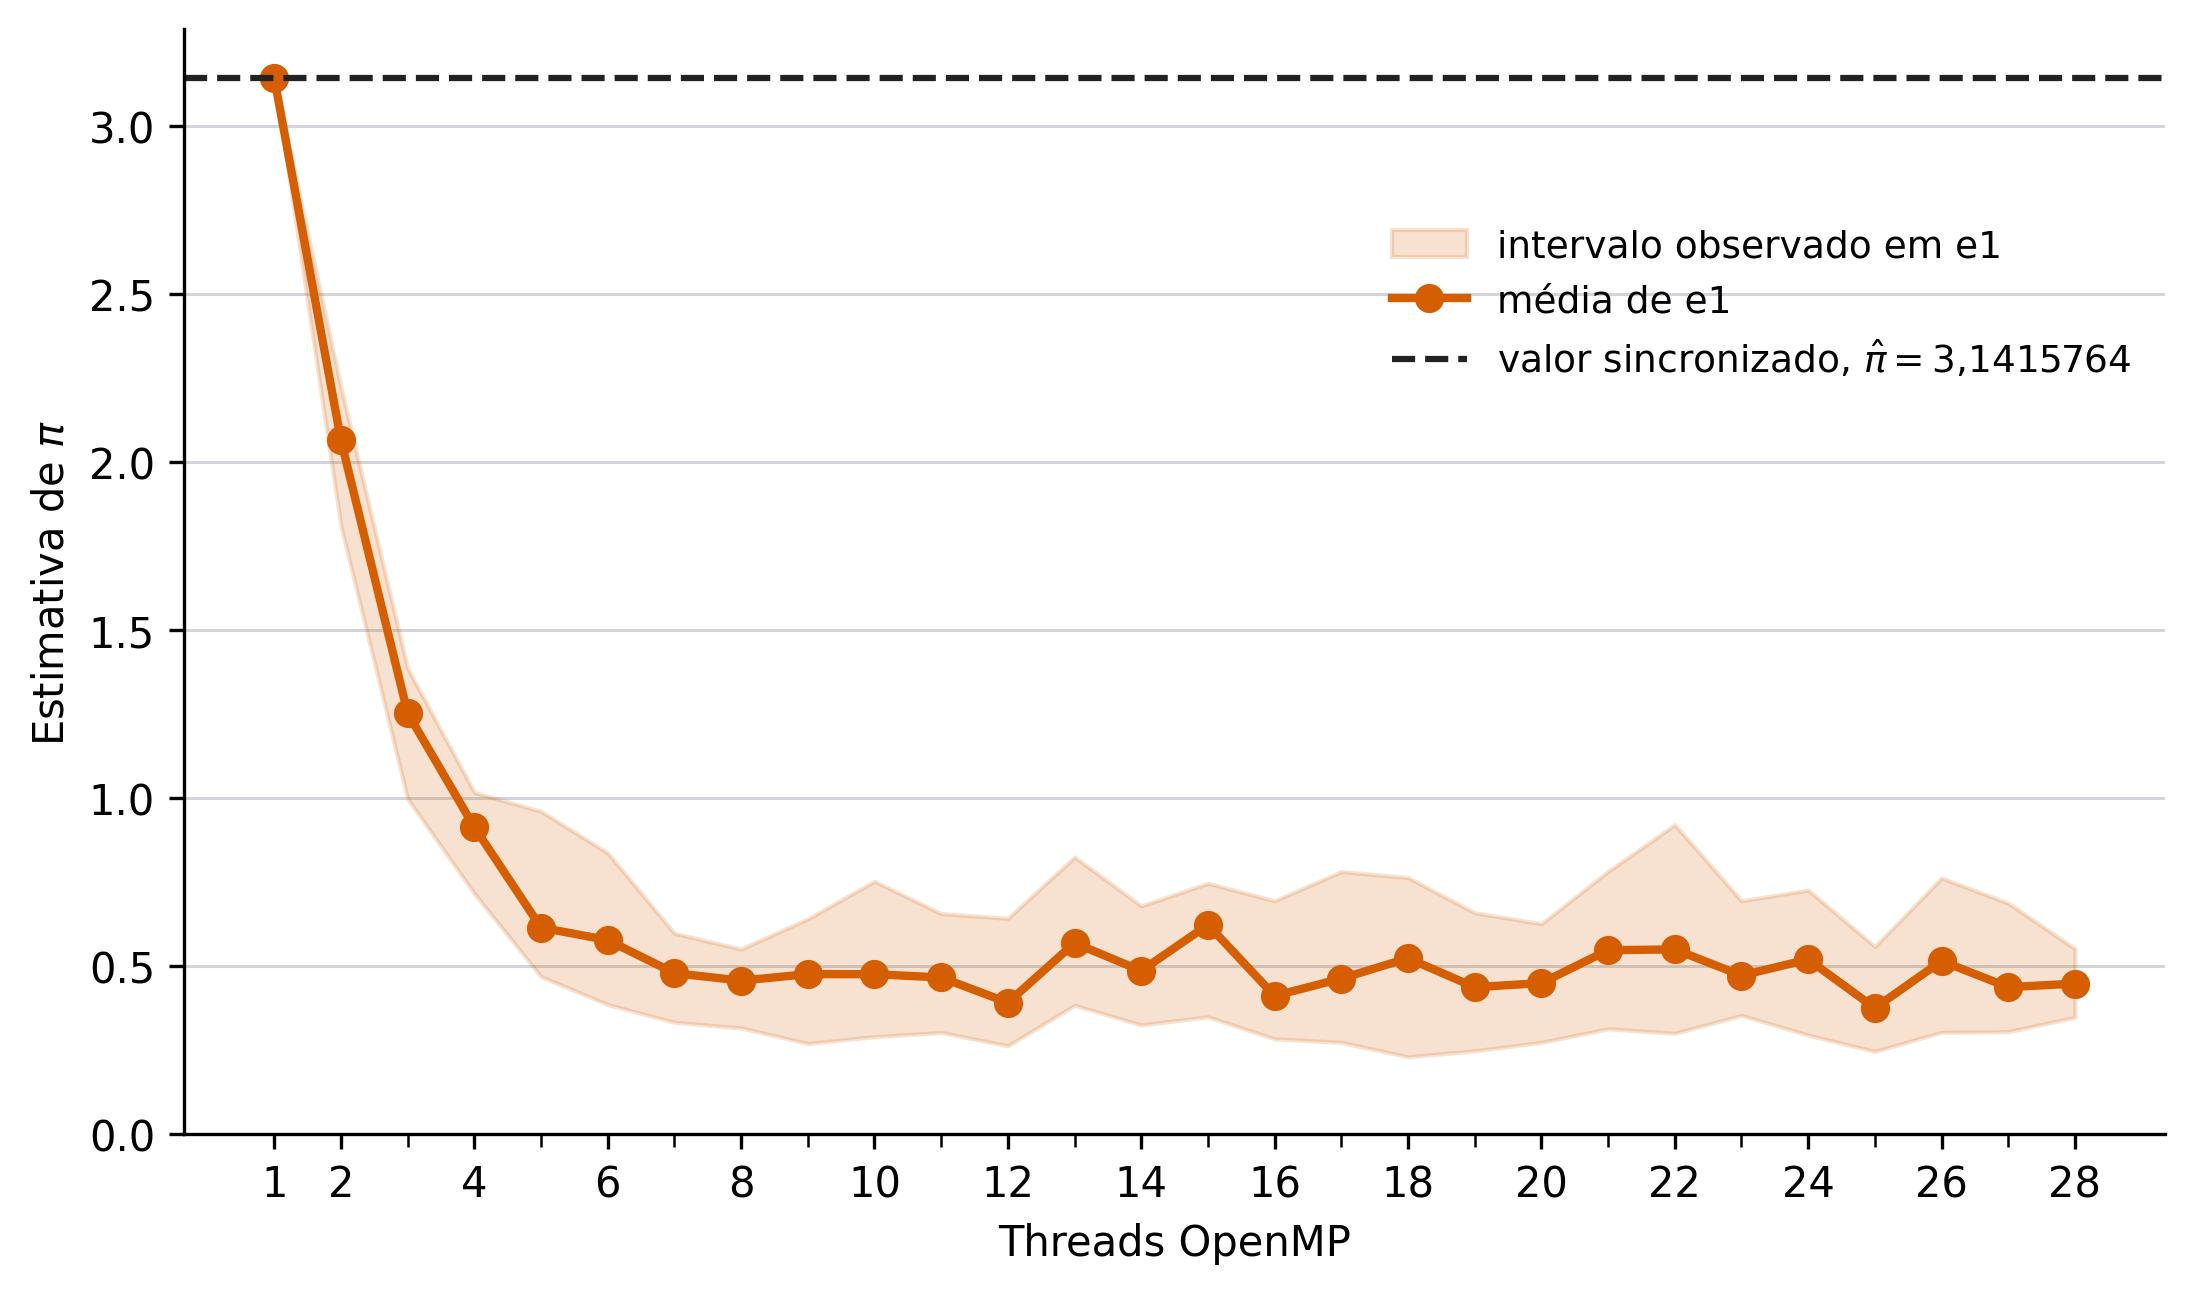
\includegraphics[width=0.9\textwidth]{race_condition_plot.png}
\caption{Média e intervalo das dez execuções de e1.c. A linha tracejada indica a estimativa sincronizada com os mesmos pontos.}
\label{fig:race}
\end{figure}

A Figura \ref{fig:race} mostra que o efeito não segue uma curva regular. A ordem das leituras e escritas muda em cada execução, portanto não há como prever quantos incrementos serão perdidos. O programa compila e termina sem falha. A comparação com uma versão sincronizada é o que revela o defeito.

\subsection{Custo da seção crítica}
A Tabela \ref{tab:tempos} compara os tempos de e2.c e e3.c. Em e2.c, o tempo mediano subiu de 0,096032 s com uma thread para 1,221722 s com 28. O trabalho geométrico é paralelo, mas aproximadamente $\pi N/4$, ou 3,93 milhões, de pontos entram no círculo e disputam a seção \texttt{critical}. Com mais threads, a disputa cresce e o tempo não cai; ele flutua entre 0,9 e 1,5 s desde a oitava thread, com desvios padrão altos.

\begin{table}[H]
\centering
\caption{Tempo mediano em segundos. A razão compara as medianas de e2.c e e3.c.}
\label{tab:tempos}
\begin{tabular}{crrr}
\hline
Threads & e2, critical por ponto & e3, contador local & Razão e2/e3 \\ \hline
1  & 0,096032 & 0,055613 & 1,73$\times$ \\
2  & 0,318125 & 0,027523 & 11,56$\times$ \\
4  & 0,570798 & 0,014342 & 39,80$\times$ \\
8  & 0,902719 & 0,009420 & 95,83$\times$ \\
14 & 0,746605 & 0,003498 & 213,44$\times$ \\
16 & 0,902004 & 0,003321 & 271,58$\times$ \\
28 & 1,221722 & 0,009430 & 129,56$\times$ \\ \hline
\end{tabular}
\end{table}

\begin{figure}[H]
\centering

\includegraphics[width=0.9\textwidth]{tempo_execucao_plot.png}
\caption{Tempo mediano de execução. As barras de erro mostram o desvio padrão de dez repetições. A escala vertical é logarítmica.}
\label{fig:tempos}
\end{figure}

Em e3.c, cada thread entra em \texttt{critical} uma vez, depois de processar o seu bloco de iterações. O tempo caiu de 0,055613 s com uma thread para 0,003498 s com 14 threads, um ganho de 15,9$\times$. Com 16 threads, o tempo foi 0,003321 s, o menor valor medido. Nas duas configurações o ganho é próximo de 16, a quantidade de threads lógicas. Com 28 threads, o tempo voltou para 0,009430 s. Nesta máquina, o melhor resultado ocorreu com os 14 núcleos físicos ou logo acima deles.

\begin{figure}[H]
\centering

\includegraphics[width=0.9\textwidth]{speedup_plot.png}
\caption{Speedup de e2.c e e3.c em relação a uma thread. A linha verde marca 14 núcleos físicos.}
\label{fig:speedup}
\end{figure}

A Figura \ref{fig:speedup} separa os dois efeitos. O speedup de e2.c fica abaixo de 1 a partir de duas threads, pois a sincronização custa mais do que o trabalho dividido economiza. Em e3.c, o speedup acompanha o número de threads até o entorno de 14 e o excesso de threads lógicas passa a competir pelos mesmos recursos de execução, aumentando o tempo e a variação.

\subsection{Comportamento das cláusulas de escopo de dados}
Quatro programas complementares foram executados para avaliar o comportamento isolado de cada cláusula de escopo:

\begin{itemize}
    \item \textbf{\texttt{private(x)}} (\texttt{e4\_private.c}): cada thread recebe uma instância não inicializada de \texttt{x} em sua pilha privada. A leitura de \texttt{x} antes de qualquer atribuição resulta em valor indefinido (lixo de memória). Ao final da região paralela, a variável externa preserva o valor original (100).
    
    \item \textbf{\texttt{firstprivate(x)}} (\texttt{e4\_firstprivate.c}): cada thread recebe uma cópia local inicializada com o valor prévio da variável (100). Modificações internas afetam apenas o escopo local de cada thread, e o valor fora da região paralela permanece 100.
    
    \item \textbf{\texttt{lastprivate(resultado)}} (\texttt{e4\_lastprivate.c}): ao término do laço paralelo de 20 iterações ($i \in [0, 19]$), a variável externa recebe deterministicamente o valor computado na última iteração lógica ($19^2 = 361$), independentemente da thread que finalizou por último.
    
    \item \textbf{\texttt{default(none)}} (\texttt{e4\_default\_none.c}): ao omitir a classificação da variável \texttt{y}, o compilador GCC detecta a variável não declarada e aborta a compilação:
    \begin{lstlisting}[language=bash]
error: 'y' not specified in enclosing 'parallel'
    \end{lstlisting}
    Esse mecanismo estático previne efeitos colaterais e corridas acidentais em programas paralelos complexos.
\end{itemize}

\section{Conclusão}
A versão e1.c mostra que um contador compartilhado não pode receber incrementos concorrentes sem sincronização. e2.c preserva a contagem, mas serializa milhões de atualizações e perde desempenho conforme o número de threads aumenta. e3.c acumula localmente e sincroniza apenas no final. Com 14 threads, a versão levou 0,003498 s, contra 0,746605 s de e2.c na mesma configuração. O teste também mostra o limite prático do hardware: depois dos 14 núcleos físicos, as threads lógicas não melhoraram o tempo de e3.c e ainda aumentaram a variância das medições.

\end{document}
